\documentclass[12pt, a4paper]{article}
\usepackage{caption}
\usepackage{graphicx}
\usepackage{hyperref}
\hypersetup{
    colorlinks,
    citecolor=black,
    filecolor=black,
    linkcolor=black,
    urlcolor=black
}
\usepackage{tikz-network}
\usepackage{amsmath, amsfonts, amssymb, amsthm}
\usepackage{algpseudocode}
\usepackage{algorithm}
\title{Network and Cybersecurity\\ Assignment 3}
\date{2022}
\author{Kristoffer Klokker}

\usepackage{xcolor,listings}
\usepackage{textcomp}
\usepackage{color}
\usepackage{listings}
\definecolor{codegreen}{rgb}{0,0.6,0}
\definecolor{codegray}{rgb}{0.5,0.5,0.5}
\definecolor{codepurple}{HTML}{C42043}
\definecolor{backcolour}{HTML}{F2F2F2}
\definecolor{bookColor}{cmyk}{0,0,0,0.90}  
\color{bookColor}
\setcounter{tocdepth}{1}
\lstset{upquote=true}

\lstdefinestyle{mystyle}{
    backgroundcolor=\color{backcolour},   
    commentstyle=\color{codegreen},
    keywordstyle=\color{codepurple},
    numberstyle=\numberstyle,
    stringstyle=\color{codepurple},
    basicstyle=\footnotesize\ttfamily,
    breakatwhitespace=false,
    breaklines=true,
    captionpos=b,
    keepspaces=true,
    numbers=left,
    numbersep=10pt,
    showspaces=false,
    showstringspaces=false,
    showtabs=false,
    tabsize=3,
}
\lstset{style=mystyle}
\usepackage{zref-base}

\makeatletter
\newcounter{mylstlisting}
\newcounter{mylstlines}
\lst@AddToHook{PreSet}{%
  \stepcounter{mylstlisting}%
  \ifnum\mylstlines=1\relax
    \lstset{numbers=none}
  \else
    \lstset{numbers=left}
  \fi
  \setcounter{mylstlines}{0}%
}
\lst@AddToHook{EveryPar}{%
  \stepcounter{mylstlines}%
}
\lst@AddToHook{ExitVars}{%
  \begingroup
    \zref@wrapper@immediate{%
      \zref@setcurrent{default}{\the\value{mylstlines}}%
      \zref@labelbyprops{mylstlines\the\value{mylstlisting}}{default}%
    }%
  \endgroup
}

% \mylstlines print number of lines inside listing caption
\newcommand*{\mylstlines}{%
  \zref@extractdefault{mylstlines\the\value{mylstlisting}}{default}{0}%
}
\makeatother


\newcommand\numberstyle[1]{%
    \footnotesize
    \color{codegray}%
    \ttfamily
    \ifnum#1<10 0\fi#1 |%
}


\begin{document}
	\maketitle
	\clearpage
	\tableofcontents
	\clearpage
	\section{Problem - Routing}
		\subsection{Give X's distance vector for destinations $W,Y$ and $U$}
			Given that $Y$, $W$ and $U$ is stable $X$s distance vector will be\\
			$c(X,Y)=min(4,6+c(W,Y),6+c(W,U)+c(U,Y))$\\
			$c(X,Y)=min(4,7,26)=4$\\
			$c(X,W)=min(6,4+c(Y,W),4+c(Y,U)+c(U,W))$\\
			$c(X,W)=min(6,5,24)=5$\\
			$c(X,U)=min(4+c(Y,U),6+c(W,U))=min(15,15)=15$
		\subsection{Give a link-cost change for either $c(X,W)$ or $c(X,Y)$ such that $X$ will inform its neighbours of a new minimum-cost path to $U$ as a result of executing the distance vector algorithm}
			For it to be announced it will require the cost to be less than the current 15, Therefore the cost change has to be less than 6 for it to be announced.
		\subsection{Give a link-cost change for either $c(X,W)$ or $c(X,Y)$ such that $X$ will not inform its neighbours of a new minimum-cost path to $U$ as a result of executing the distance vector algorithm}
			Since bad news travels slow, a cost change larger than 6 will result in $X$'s route to $U$ not being updates and it will not announce any changes.
	\clearpage
	\section{Problem - IPsec}
		Describe two scenarios where SDU would use IPsec.\\
		Two examples of use of IPsec by SDU is SDU VPN which enables remote access to the SDU network and the SDU mail server.\\
		The SDU VPN can be connected to using IPsec, for the connection to be encrypted the VPN will be using tunnel mode with ESP. The tunnel mode is used since it will go through multiple routers to get to this host. The ESP is used for the encryption of the connection.\\
		Another use would be for authentication for services which encryption is not needed. Here the AH service model protocol can be used, this would be favorable since the firewall can use it for package sorting.
	\section{Problem - DHCP}
		\subsection{Network administrator Anders is new to the organisation, and is semi-obsessed with redundancy. Anders would like to have two DHCP servers on his company network. If Anders installs a second DHCP server on the network, your laptop when joining the network would receive offers from the two different DHCP servers. Argue if this would work or not}
			This would work fine, the laptop will simply respond to the wanted DHCP server from the two given request.\\
			Since the laptop will issue the request at 255.255.255.255 every DHCP server will get the request and answer back at the same address.\\
		\subsection{Is there something Anders should remember to do to make the scenario in a) work}
			The two DHCP servers should have different IP addresses, such when answering the request the correct DHCP server get the response.\\
			Also must the DHCP servers ip range not overlap. This is to ensure that the DHCP server does not give out the same IP address to two different devices.
		\subsection{If a power outage happens at Anders organisation, all machines would start again at the same time. How would this affect the DHCP server(s)? Is there anything the DHCP clients could/should do to alleviate this issue?}
			To ensure no confusion could happen the DHCP servers IP address on the network should be static, if the DHCP servers IP is not static, the clients would fail to renew their IP, and then send a discover package instead.\\
			The DHCP servers should have saved the lease data in a persistent storage, therefore it should be able go back to where it left off.
		\subsection{Draw a timing diagram for the scenarios.}
			In the two scenarios have I used the DHCP example where:\\
			\begin{itemize}
				\item The DHCP server IP is 192.0.0.1
				\item The offered IP is 192.0.0.2
				\item The first transaction has id 1 and the second is id 2
			\end{itemize}
			\subsubsection{The DHCP discover message is lost.}
				\begin{figure}[h!]
					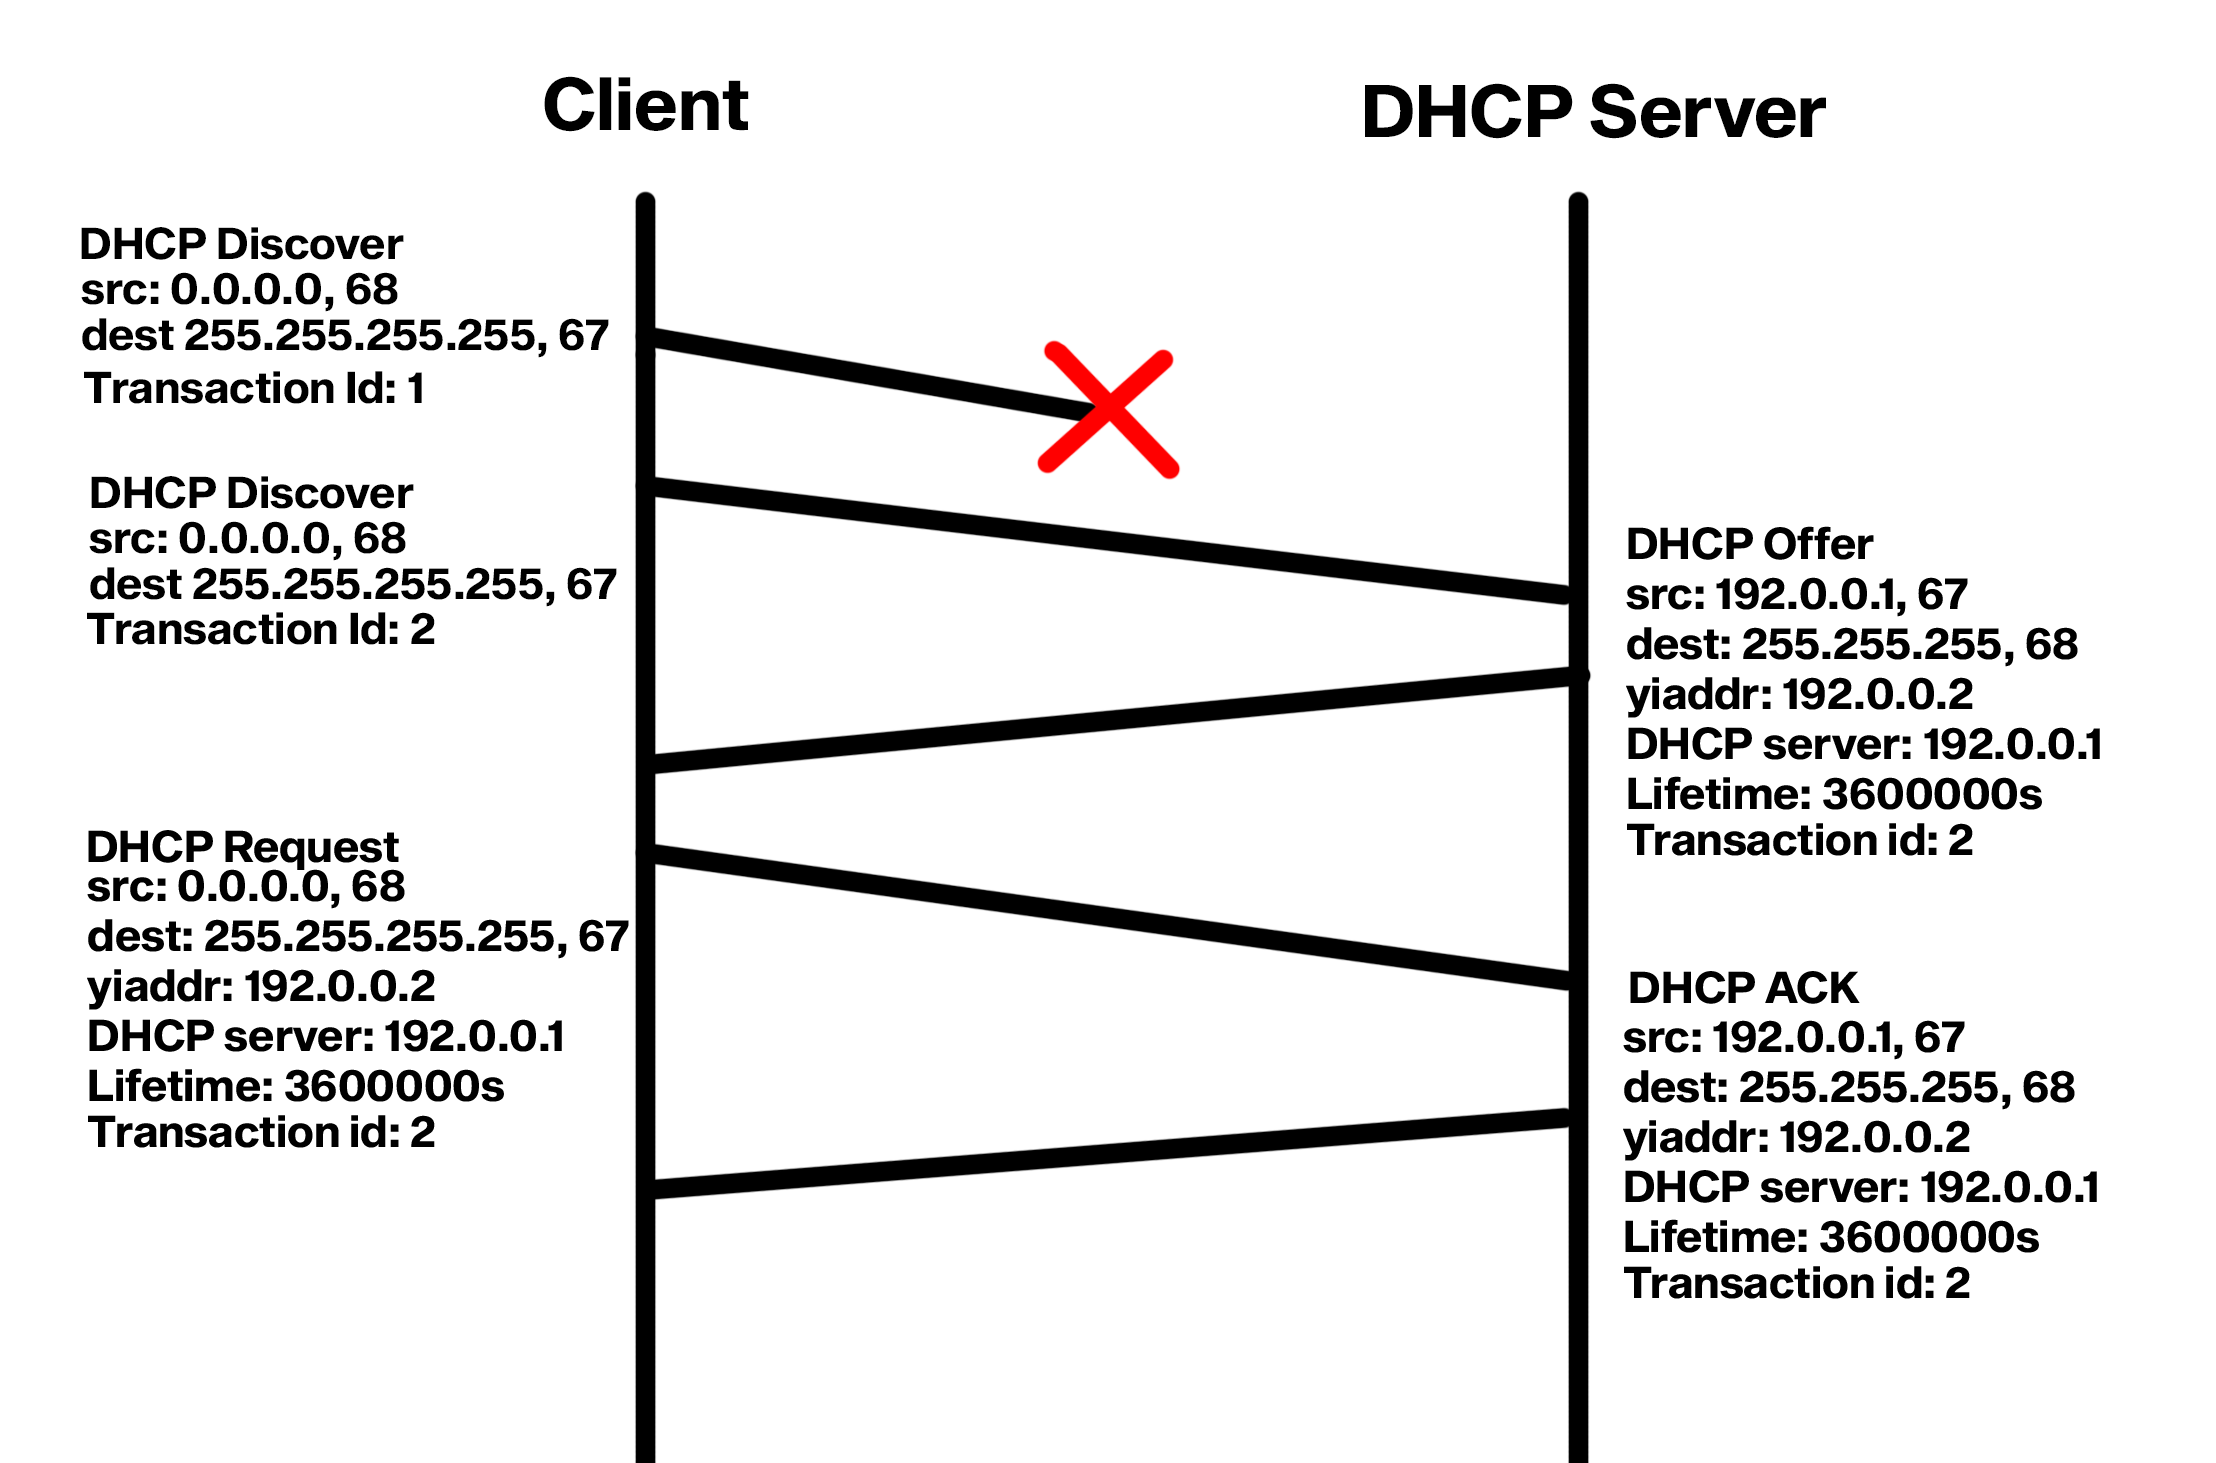
\includegraphics[width=300px]{assets/dhcp1.png}
					\caption{DHCP timing diagram where the first discover package is lost}
				\end{figure}
				The time between the two discover messages is defined in dhcpclient.conf file on linux systems.
			\subsubsection{The DHCP offer message is lost}
				\begin{figure}[h!]
					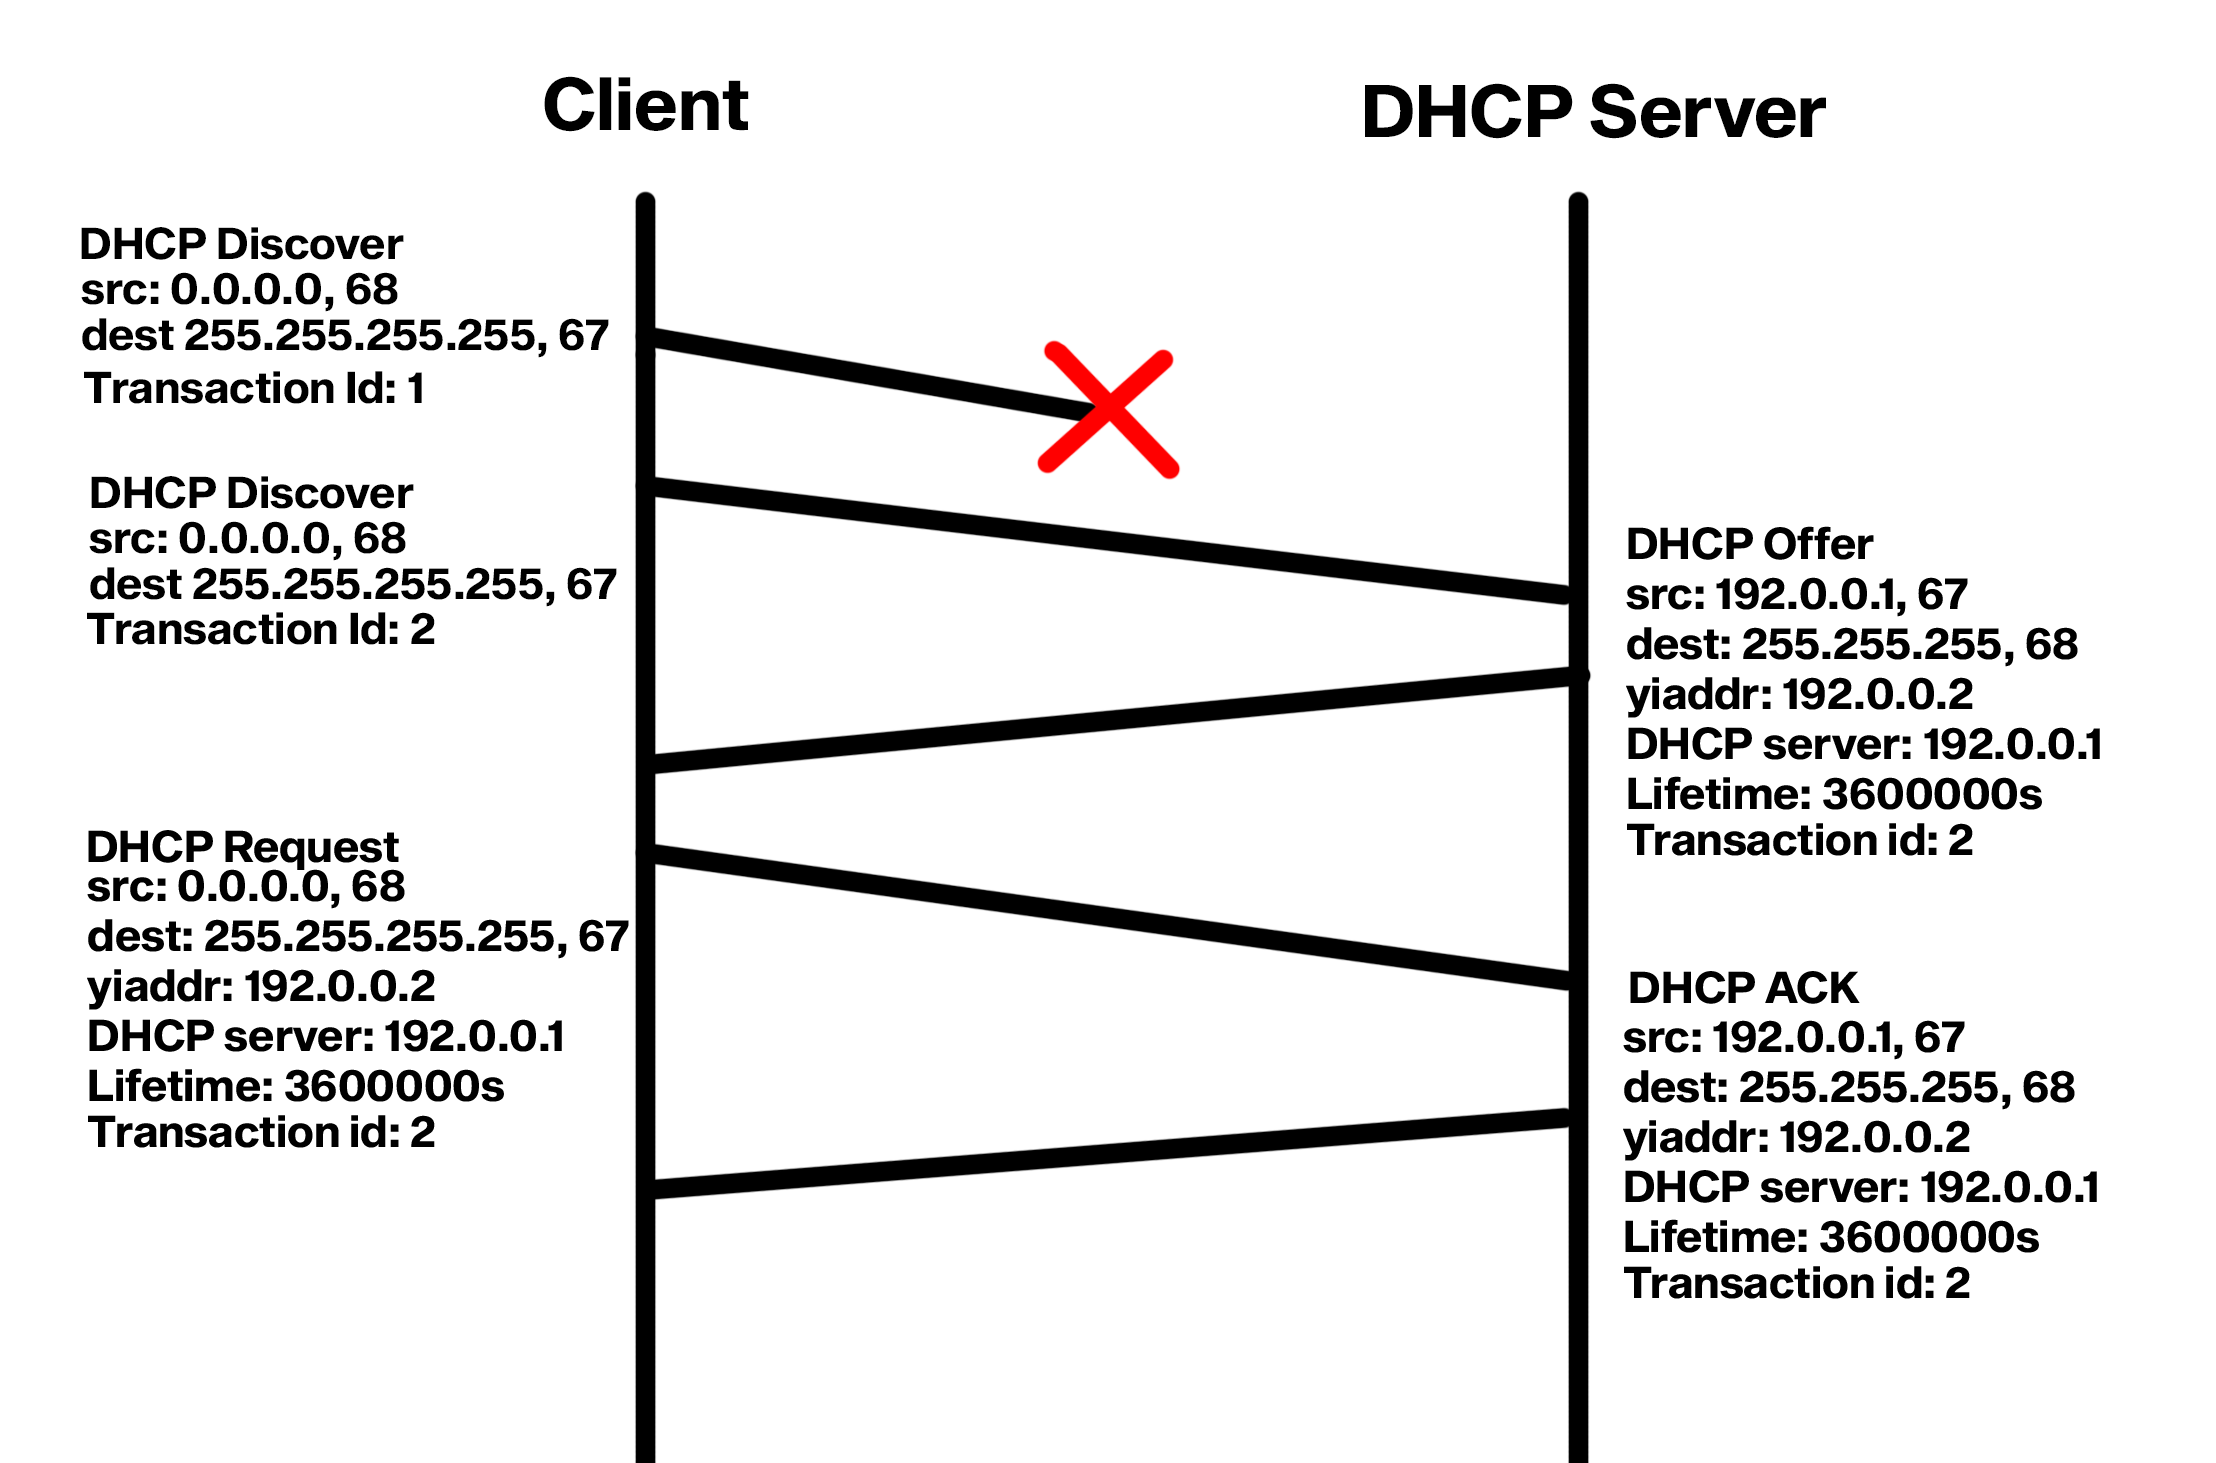
\includegraphics[width=300px]{assets/dhcp1.png}
					\caption{DHCP timing diagram where the first discover package is lost}
				\end{figure}
				The time between the two discover messages is again the defined time.\\
				From the server perspective have it never gotten an acknowledgement and therefore the IP is still open.
				
			
			 
\end{document}
